\section{Introduction}
\label{sec:introduction}

\tk{TODO}

\tk{Mention:
\begin{itemize}
\item Using natural units
\item Using the assumption that production and decay of the Higgs are decoupled
\end{itemize}
}

\tk{%
Place the combination plot with all the decay channels / production modes here; makes a nice argument about the usefulness of differential measurements.
}

As exemplified in Fig.~\ref{fig:productiondecay}, inclusive measurements~\cite{%
Khachatryan:2016vau,% 7 & 8 TeV coupling combination
Aad:2015zhl,% 7 & 8 TeV mass combination
Sirunyan:2018koj% 13 TeV CMS coupling combination
}
have thus far not shown any deviation from the SM prediction.
% 


\begin{figure}[hbtp]
  \begin{center}
    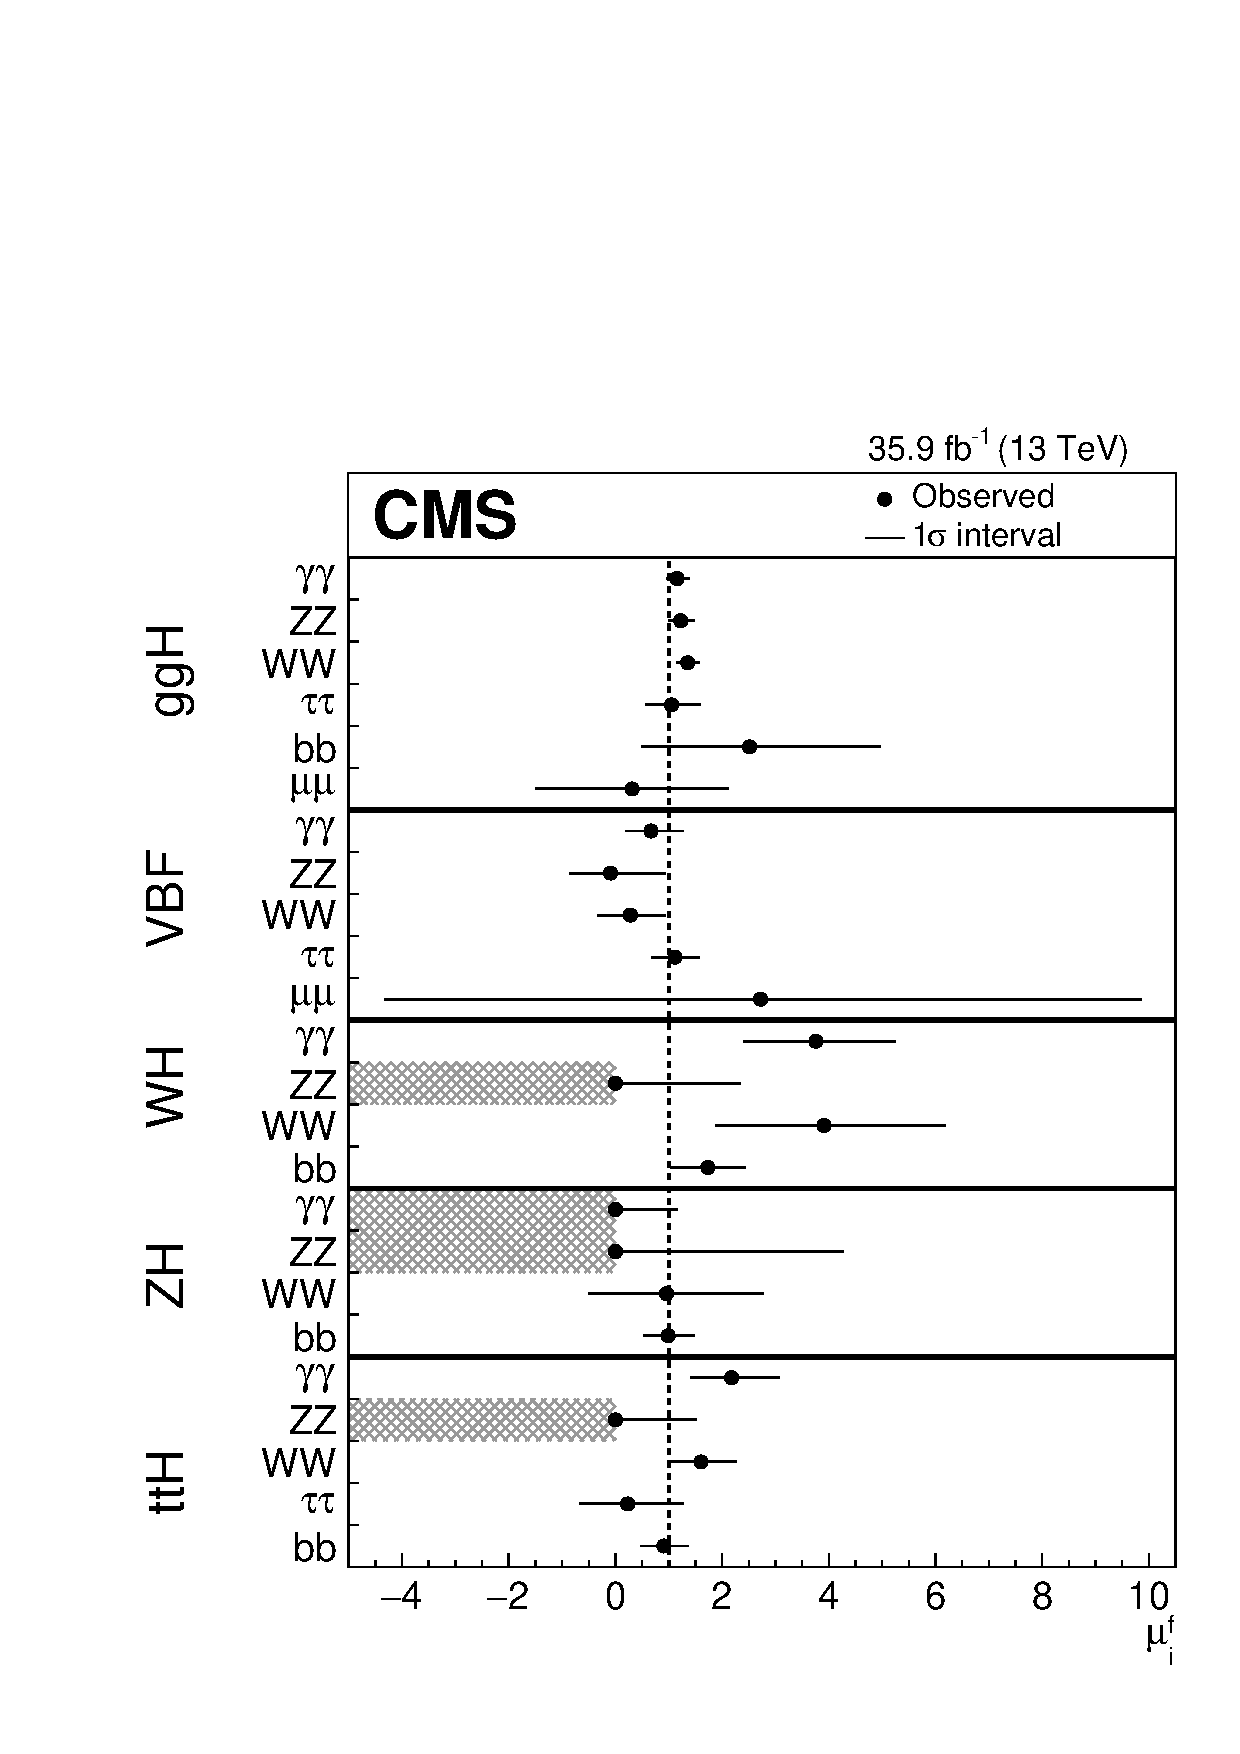
\includegraphics[width=0.7\linewidth]{img/theory/grandcomb/productiondecay.pdf}
    \caption{
        Taken from Ref.~\cite{Sirunyan:2018koj}.
        }
    \label{fig:productiondecay}
  \end{center}
\end{figure}


Given that the vast majority of detectors nowadays have a cylindrical design, particle kinematics are typically described in geometrically-related coordinates: The \textit{energy} $E$ of the particle, the \textit{transverse momentum} $\pt$, the rapidity $y$, and the azimuthal angle $\phi$.
% 
A quantity closely related to $y$ is the pseudorapidity $\eta$, which in the high energy limit approaches $y$, but has the advantage of needing only the angle with respect to the beamline to be computed.



The kinematics of the Higgs boson are fully described by $\mh$, $\absy$ and $\pth$.
% 
The $\absy$ distribution is determined mostly by the gluon PDF; while interesting as a potential constrain on the gluon PDF in a global PDF fit, it is of limited value in the context of Higgs boson property measurements.
% 
In order for $\pth$ to be non-zero, the production of the Higgs boson has to be associated with some other particle to recoil off of, which in the case of $\ggh$ naturally occurs via QCD radiation.





As the dominant Higgs boson production mode at the LHC is $\ggh$, the predictions of differential distributions are given primarily by the predictions of $\ggh$.
% 
Because of the loop in the LO $\ggh$ diagram, the $\pth$ distribution of Higgs bosons produced via $\ggh$ is a good probe for new physics and potentially a portal towards precision measurements of the Higgs boson properties, for the following reasons.
% 
Firstly, up until now, the loop has not been observed experimentally; Confirming its existence is an important verification of the SM.
% 
Secondly, the couplings of the Higgs boson to other SM particles can affect the shape of differential distributions while preserving the overall normalization.
% 
By fitting the shape of theoretical predictions under simultaneous variations of Higgs boson couplings to the shape observed in data, the Higgs boson couplings can be further constrained.
% 
And thirdly, if there any heavy BSM particles in the loop, the tails of the $\pth$ are expected to deviate with respect to their SM values.
% 
As the tails concern only a small part of the inclusive cross section, these deviations would be hard to observe in an inclusive cross section measurement.
% 
This thesis is concerned with the first two points, although the applied methodology would as well be suitable for a search of heavy particles in the $\ggh$ loop.







% 
In the case of Higgs boson production via gluon fusion, finite quark mass effects and moderate variations to Higgs boson couplings may manifest themselves through distortions of the $\pth$ spectrum.

